%% 
%%	This is file 'beamer_sample.tex'
%%	according to an MPIDR's PowerPoint template (?)
%%	
%%	by Eric Naujoks
%%
%%	Problems, bugs and comments to 
%%	naujoks@demogr.mpg.de
%%

%%%%%%%%%%%%%%%%%%%%%%%%%%%%%%%%%%
%%	Praelegomena								%%
%%%%%%%%%%%%%%%%%%%%%%%%%%%%%%%%%%
%%	- Make sure that you use utf8-encoding for all your .tex-files!!! (TeXnicCenter since version 2.0)
%%	- TeXnicCenter update: MPIDR intranet > Hard- & Sortfware > Software > Script and text editors > TeXnicCenter

\documentclass[20pt]{beamer}

\usepackage[ngerman,english]{babel}
\usepackage{tikz}
\usepackage[normalem]{ulem}
\geometry{paperwidth=10in, paperheight=7.5in}
\usepackage{animate}
\usepackage{array}

\usepackage[utf8]{inputenc}

\usepackage[mpidr]{./mpidr/beamerthemeMPIDR}

%% Declaring title and author
\title{Morbidity compression}
\subtitle{Tim Riffe}		%%

%%	the institute's logo
\renewcommand{\mylogo}{\includegraphics[width=4.7in]{mpidr_logo_colour_en}}
\usepackage{color}
\definecolor{mygray}{rgb}{0.8,0.8,0.8}

\defbeamertemplate{description item}{align left}{\insertdescriptionitem\hfill}
%%	should be the very last package to be loaded
\usepackage{hyperref}

%%%%%%%%%%%%%%%%%%%%%%%%%%%%%%%%%%
%%	Beginning of the document		%%
%%%%%%%%%%%%%%%%%%%%%%%%%%%%%%%%%%
\begin{document}

%%	titlepage - fixed frame:
%%	========================

\begin{frame}
	\titlepage
\end{frame}
%-------------------

\begin{frame}
	\frametitle{Shout-outs}
	\begin{block}{This work is a spin-off from papers with:}
	Paul Chung, John MacInnes, Jeroen Spijker, Alyson van Raalte, Maarten Bijlsma
	\end{block}
	One or more of them may also join in the present work, but blame me for today's
	ideas.
\end{frame}

\begin{frame}
\frametitle{Fries' diagrams are a nice prop}
\begin{center}
  \begin{tikzpicture}
    \node<1> (img1)
    {\includegraphics[width=.8\linewidth]{Figures/FriesFigure1.pdf}}; 
  \end{tikzpicture}
\end{center}
\end{frame}


\begin{frame}
\frametitle{Pattern indifference within lifespan}
\begin{center}
  \begin{tikzpicture}
    \node<1> (img1)
    {
\includegraphics[width=.9\linewidth]{Figures/boxflip1.pdf}}; 
    \node<2>
    (img2) {
\includegraphics[width=.9\linewidth]{Figures/boxflip2.pdf}}; 
  \end{tikzpicture}\\ \vspace{5cm}
  (if we all died at the same age then this stuff would be easy)
\end{center}

\end{frame}
\begin{frame}
\frametitle{Patterns matter if lifespans are mixed}
\begin{center}
  \begin{tikzpicture}
    \node<1> (img1)
    {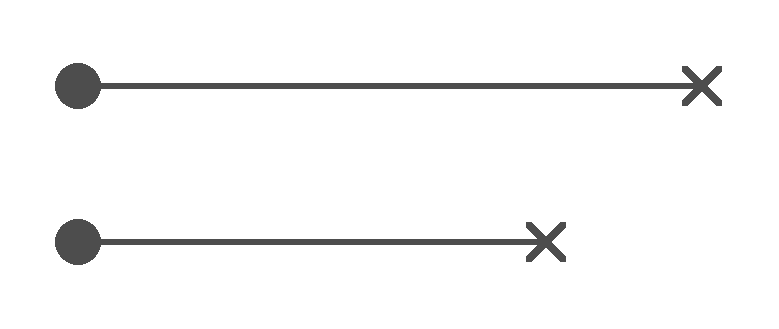
\includegraphics[width=.7\linewidth]{Figures/lifelines1.pdf}}; 
    \node<2>
    (img2) {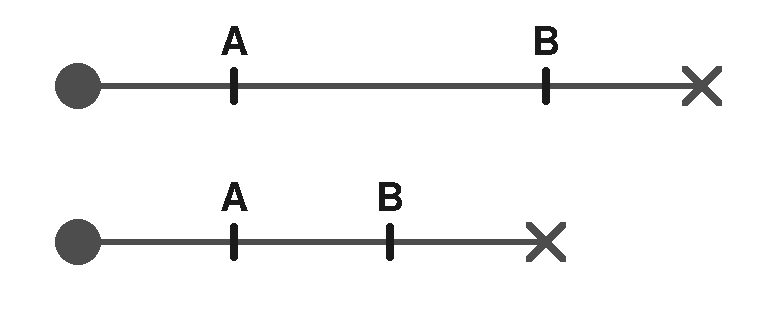
\includegraphics[width=.7\linewidth]{Figures/lifelines2.pdf}}; 
    \node<3> (img3) {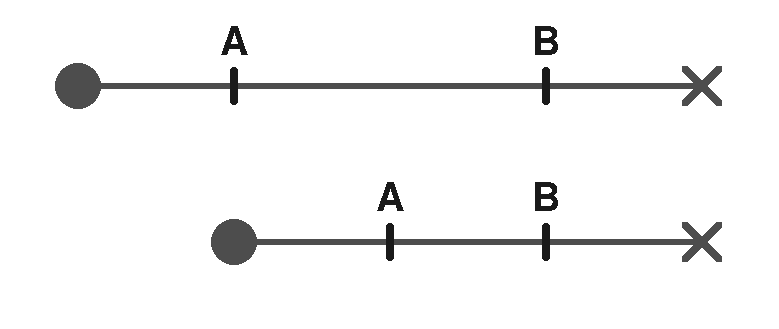
\includegraphics[width=.7\linewidth]{Figures/lifelines3.pdf}};
  \end{tikzpicture}
\end{center}
\end{frame}


\begin{frame}
\frametitle{Patterns matter if lifespans are mixed}
\begin{center}
  \begin{tikzpicture}
    \node<1> (img1)
    {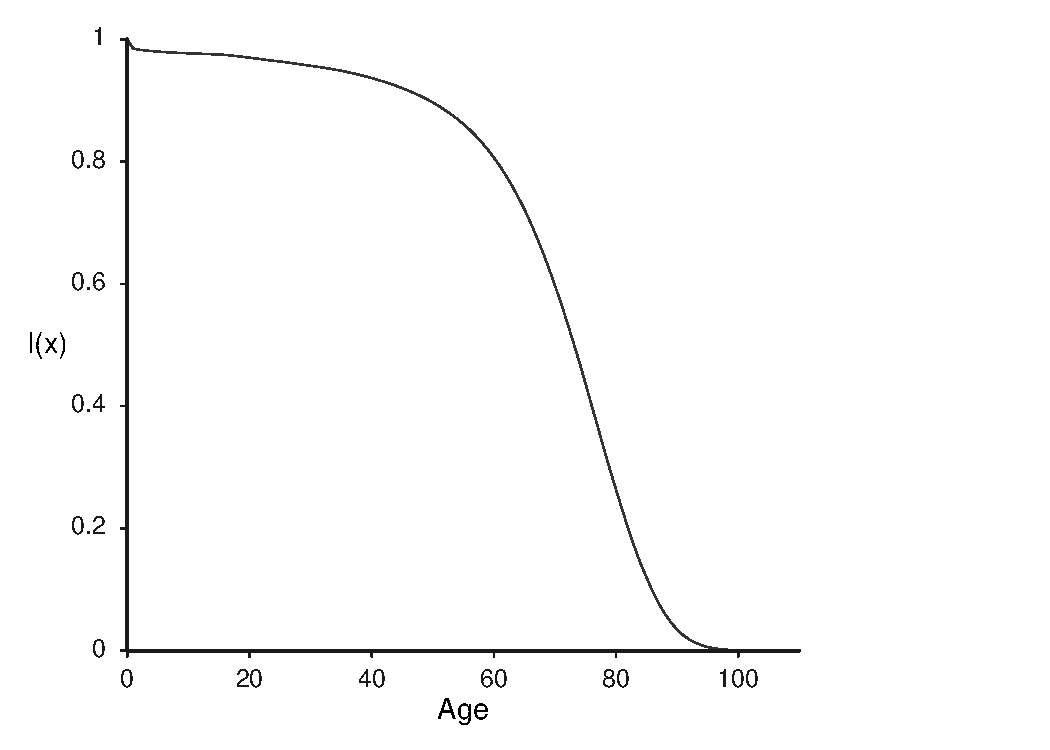
\includegraphics[width=.9\linewidth]{Figures/Japan1.pdf}}; 
    \node<2>
    (img2) {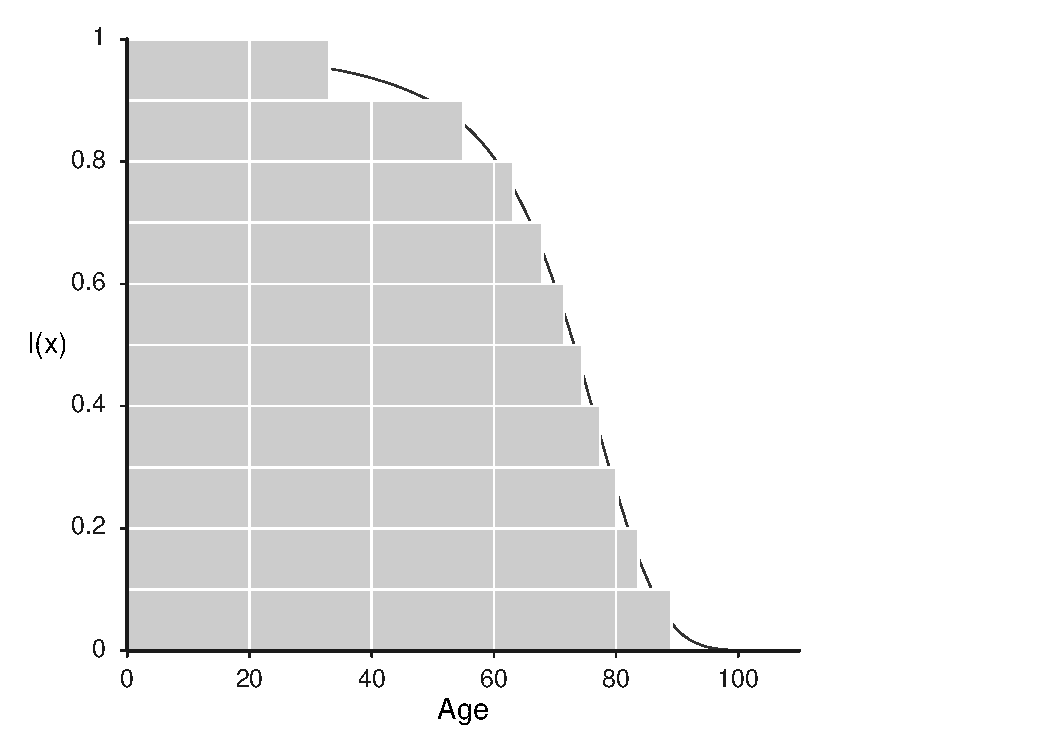
\includegraphics[width=.9\linewidth]{Figures/Japan2.pdf}}; 
     \node<3>
    (img3) {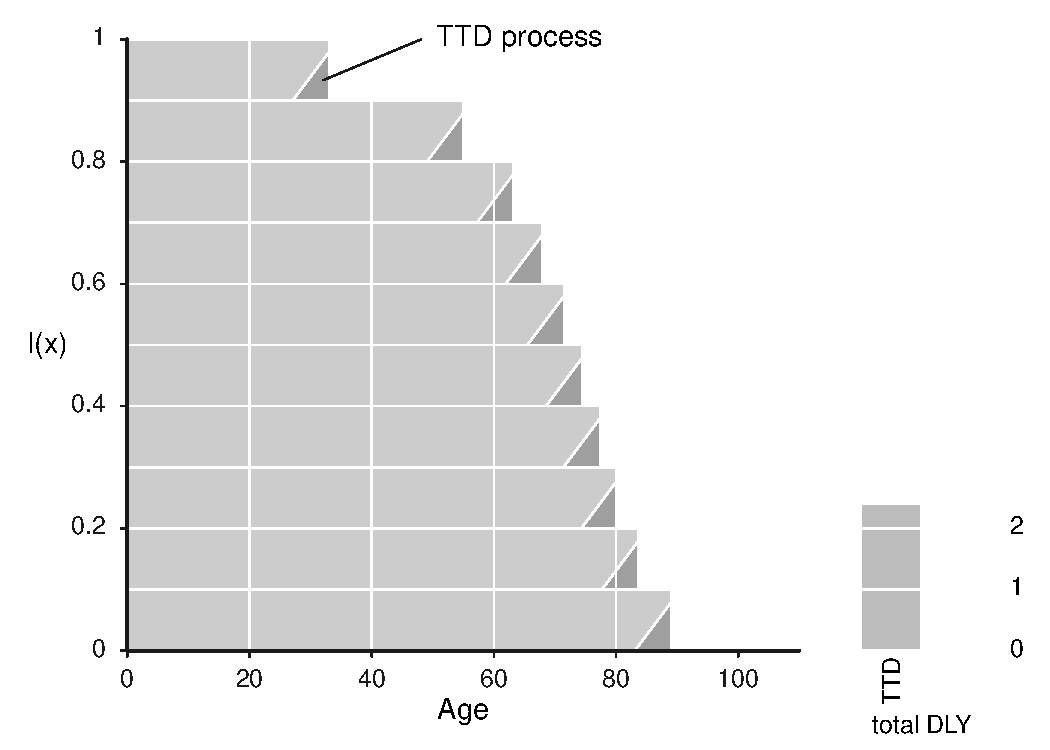
\includegraphics[width=.9\linewidth]{Figures/Japan3.pdf}}; 
    % \node<4>
   % (img4) {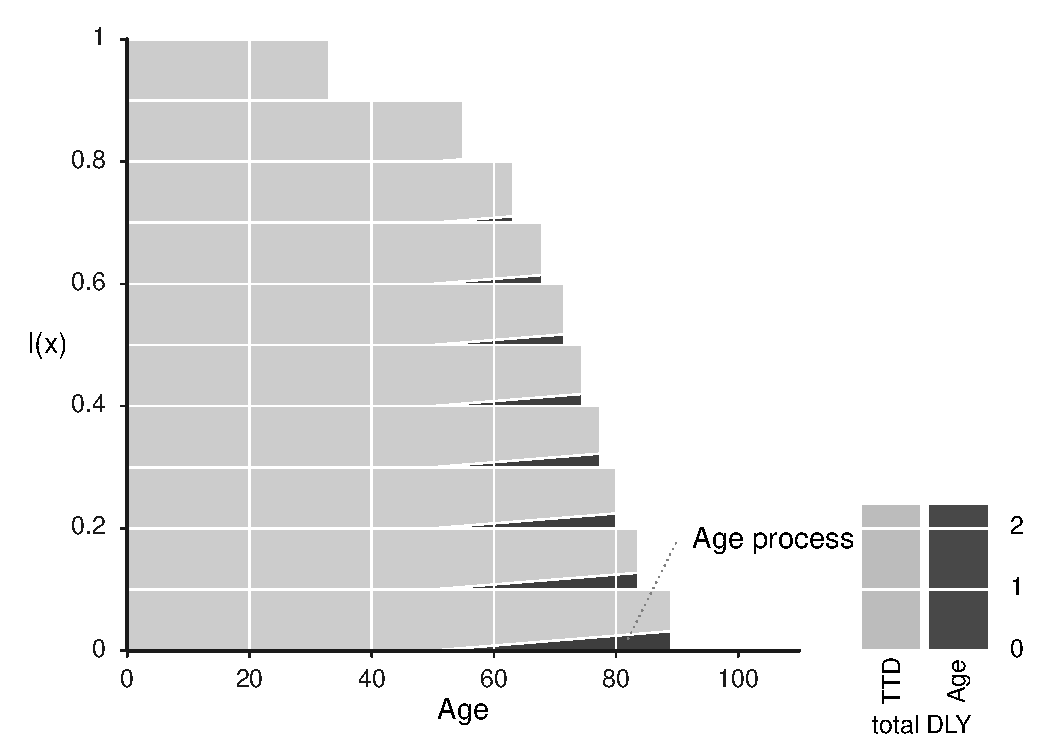
\includegraphics[width=.9\linewidth]{Figures/Japan4.pdf}}; 
     \node<4>
    (img4) {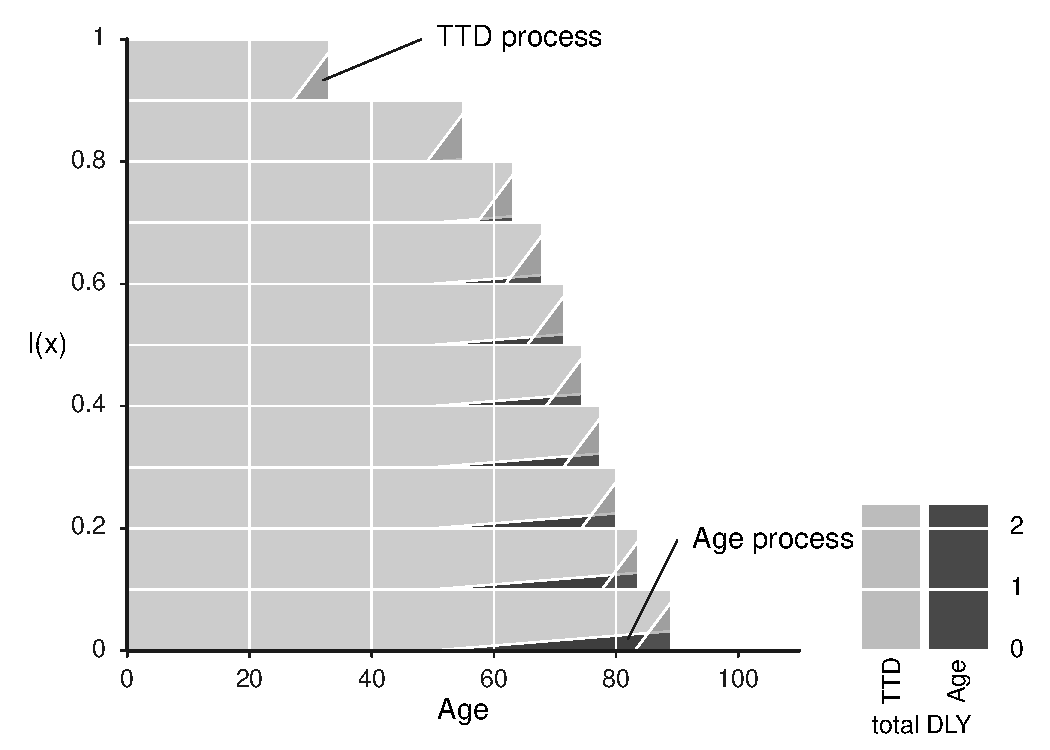
\includegraphics[width=.9\linewidth]{Figures/Japan5.pdf}}; 
     \node<5>
    (img5) {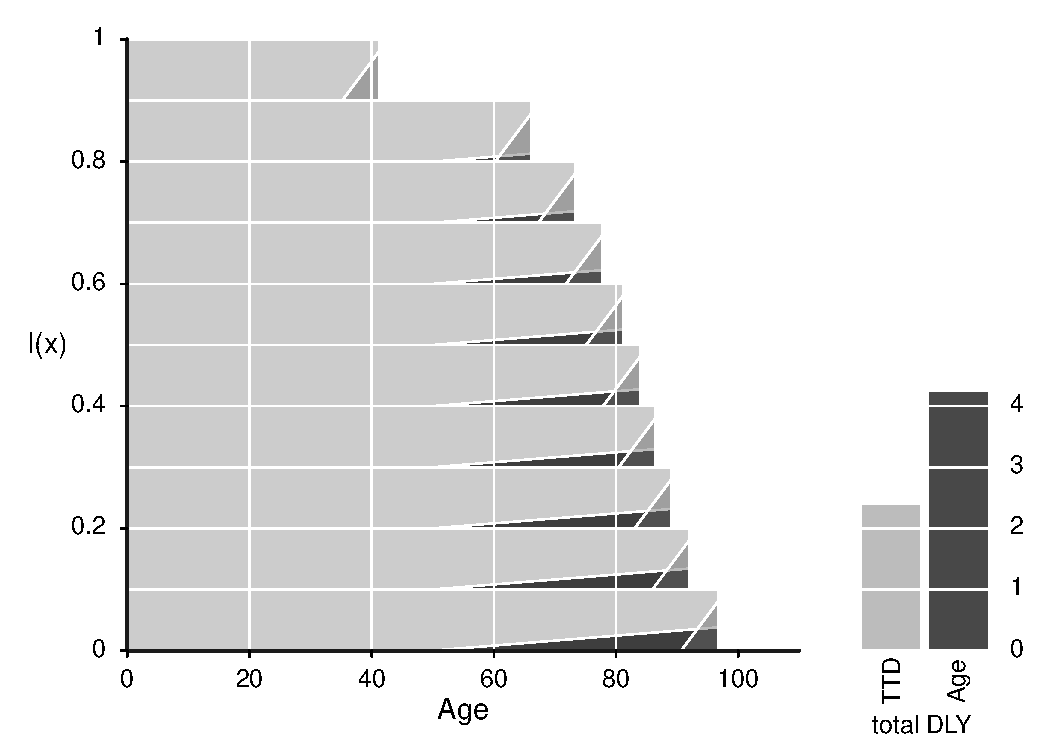
\includegraphics[width=.9\linewidth]{Figures/Japan6.pdf}}; 
  \end{tikzpicture}
\end{center}
\end{frame}

\begin{frame}
\frametitle{Compression}
\begin{block}{Complaint:}
Although neither morbidity pattern changed, standard measures would conclude
that the TTD morbidity compressed, and the age-pattern did not. DLY says nothing
of concentration in the morbidity pattern.
\end{block}

\begin{block}{Objective:}
Separate morbidity levels and morbidity concentration.
\end{block}
\end{frame}

\begin{frame}
\frametitle{Fries' diagrams are ignored in practice}
\begin{center}
  \begin{tikzpicture}
    \node<1> (img1)
    {\includegraphics[width=.8\linewidth]{Figures/FriesFigure1.pdf}}; 
    \node<2>
    (img2) {\includegraphics[width=.8\linewidth]{Figures/FriesFigure2.pdf}}; 
  \end{tikzpicture}
\end{center}
\end{frame}

\begin{frame}
\frametitle{Schematic time-to-death patterns}
\vspace{-2em}
\begin{center}
  \begin{tikzpicture}
    \node<1> (img1)
    {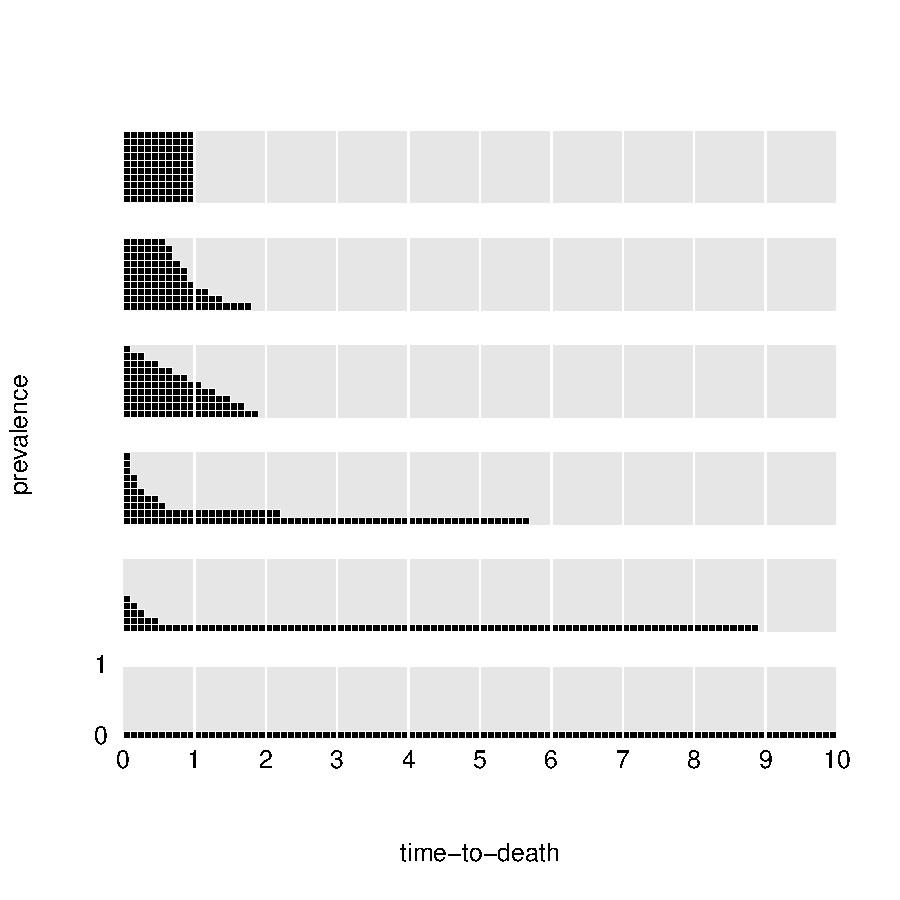
\includegraphics[width=.8\linewidth]{Figures/CompareTTD1.pdf}}; 
    \node<2>
    (img2) {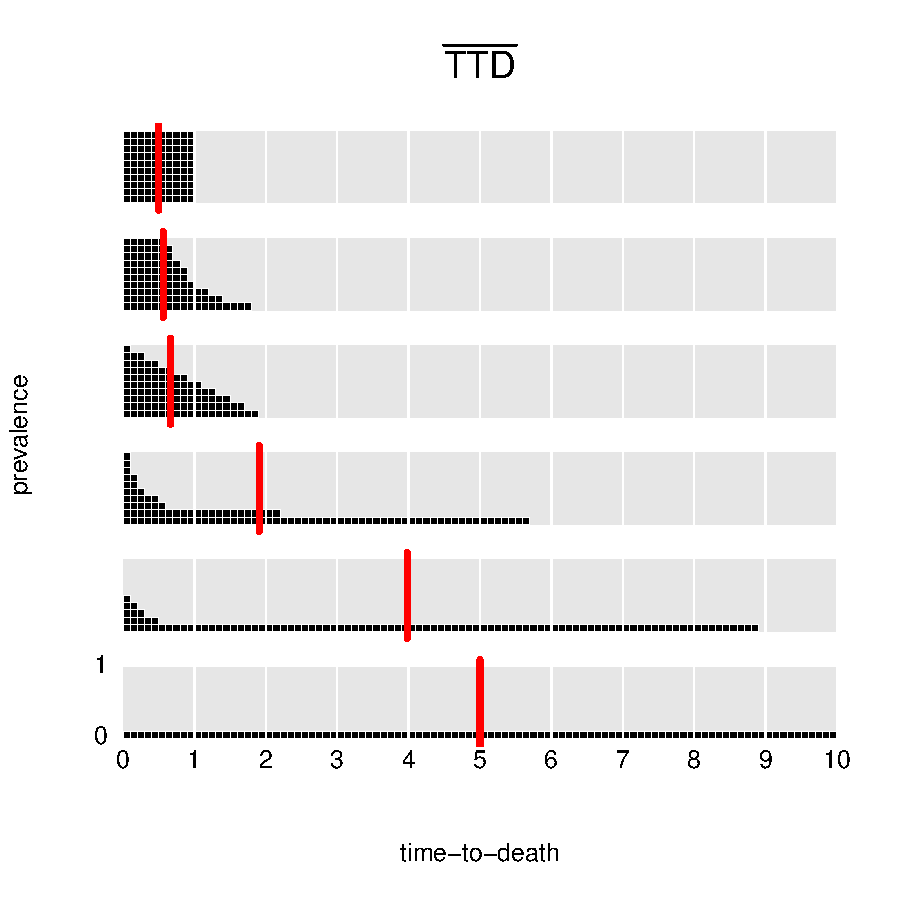
\includegraphics[width=.8\linewidth]{Figures/CompareTTD2.pdf}}; 
    \node<3>
    (img3) {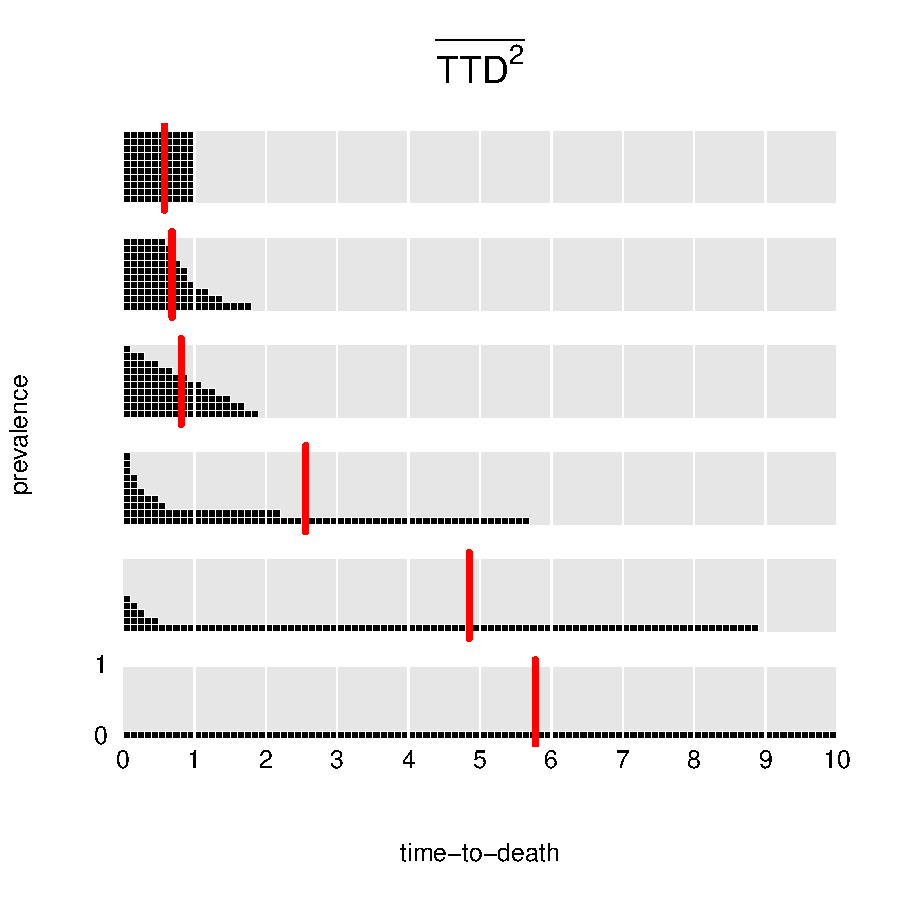
\includegraphics[width=.8\linewidth]{Figures/CompareTTD3.pdf}}; 
    \node<4>
    (img4) {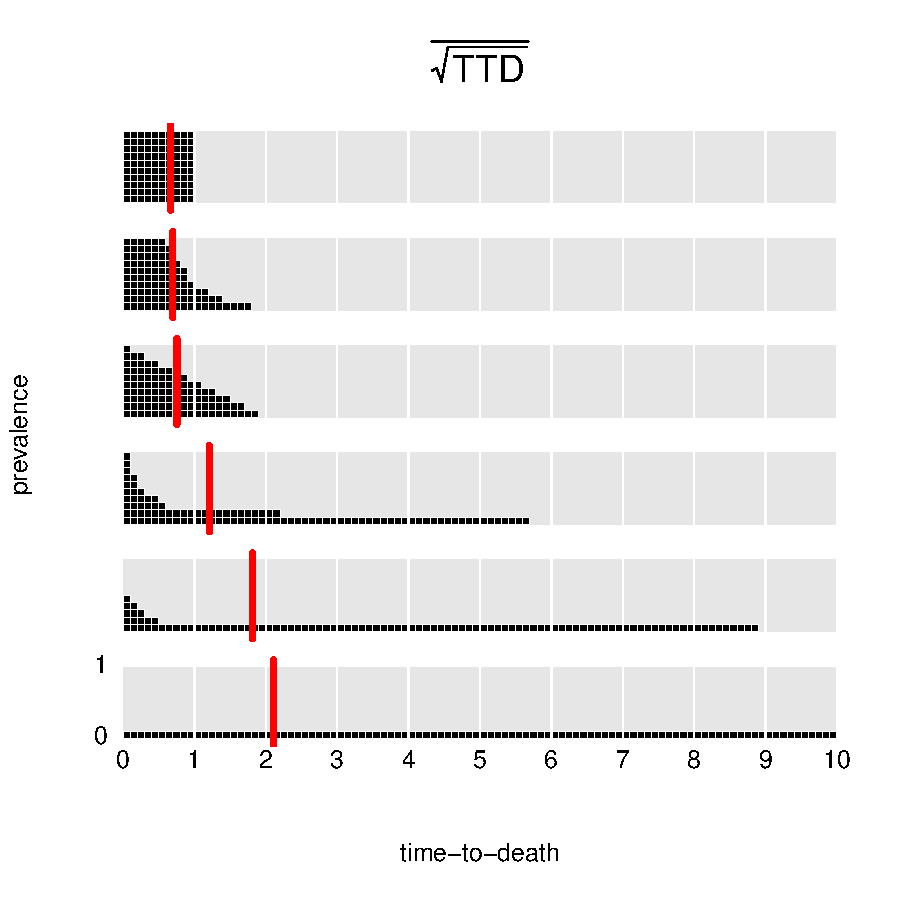
\includegraphics[width=.8\linewidth]{Figures/CompareTTD4.pdf}}; 
  \end{tikzpicture}
\end{center}
\end{frame}

\begin{frame}
\frametitle{Real time-to-death patterns (HRS, ADL3)}
\vspace{-1em}
\begin{center}
  \begin{tikzpicture}
    \node<1>  (img1) {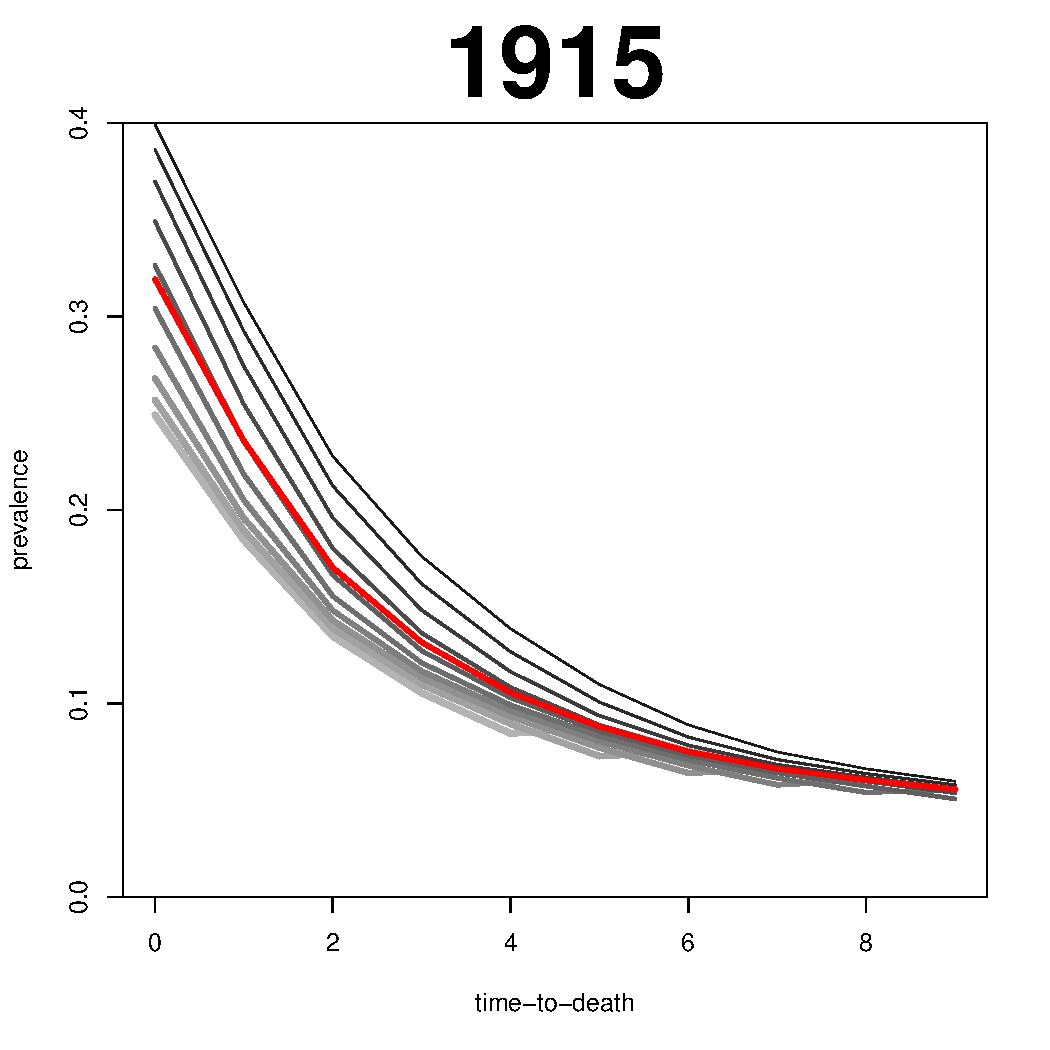
\includegraphics[width=.7\linewidth]{Figures/adl31915.pdf}}; 
    \node<2>  (img2) {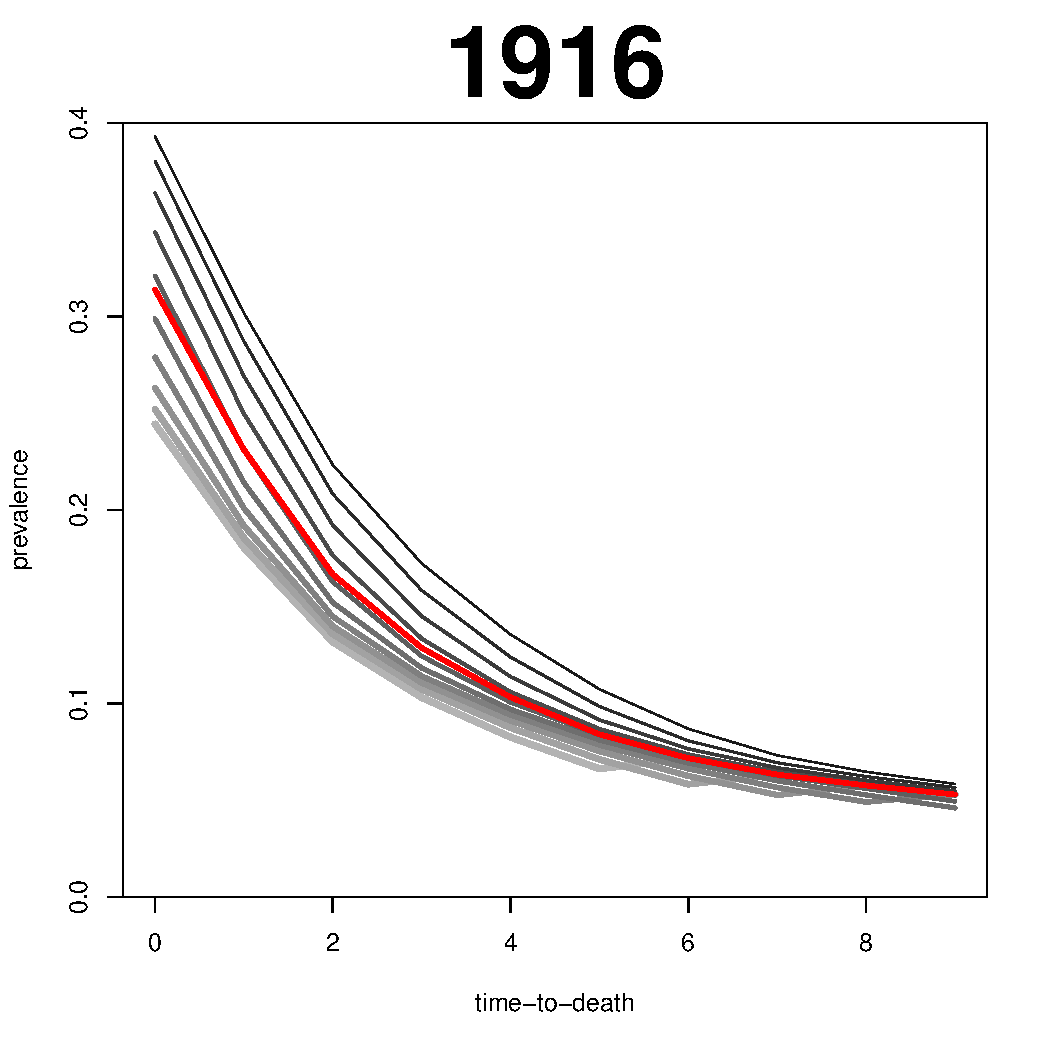
\includegraphics[width=.7\linewidth]{Figures/adl31916.pdf}}; 
    \node<3>  (img3) {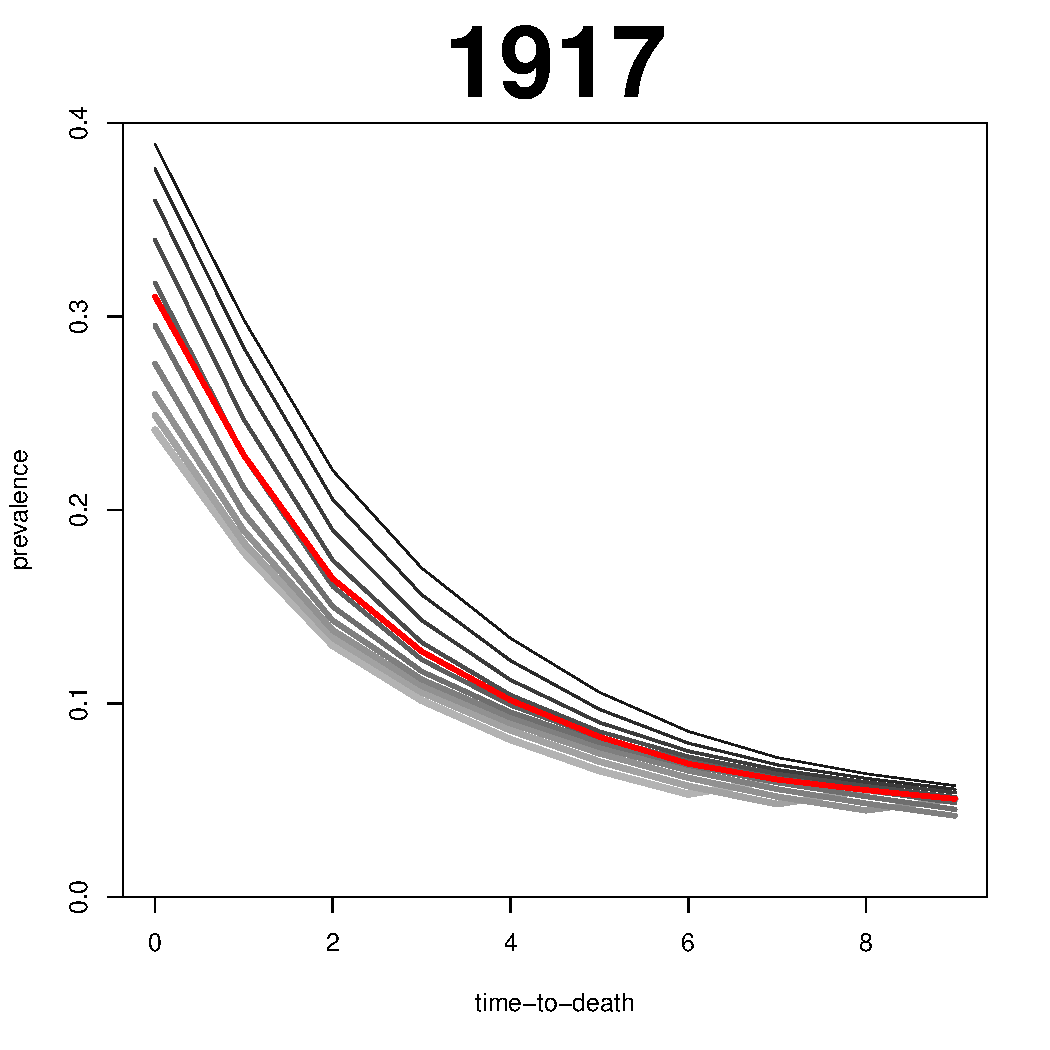
\includegraphics[width=.7\linewidth]{Figures/adl31917.pdf}}; 
    \node<4>  (img4) {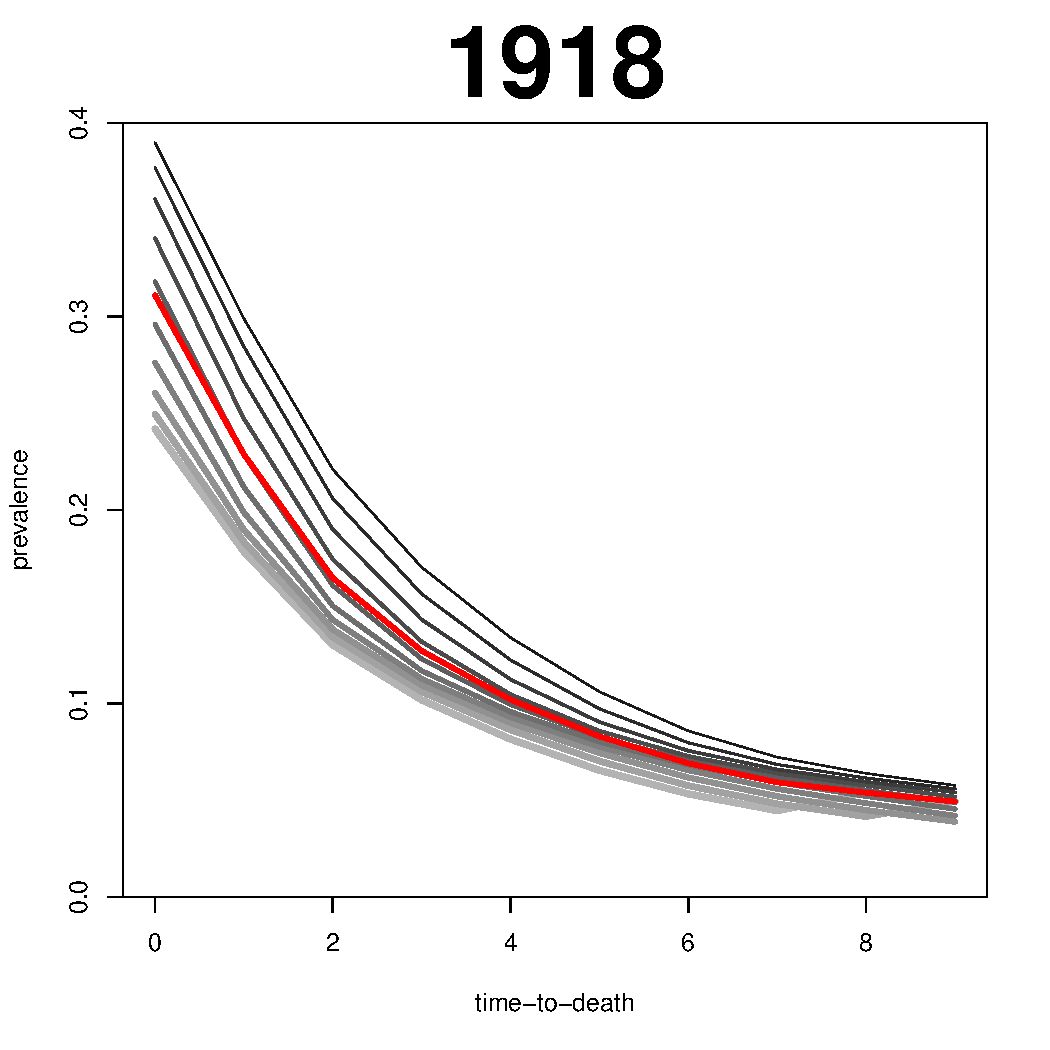
\includegraphics[width=.7\linewidth]{Figures/adl31918.pdf}}; 
    \node<5>  (img5) {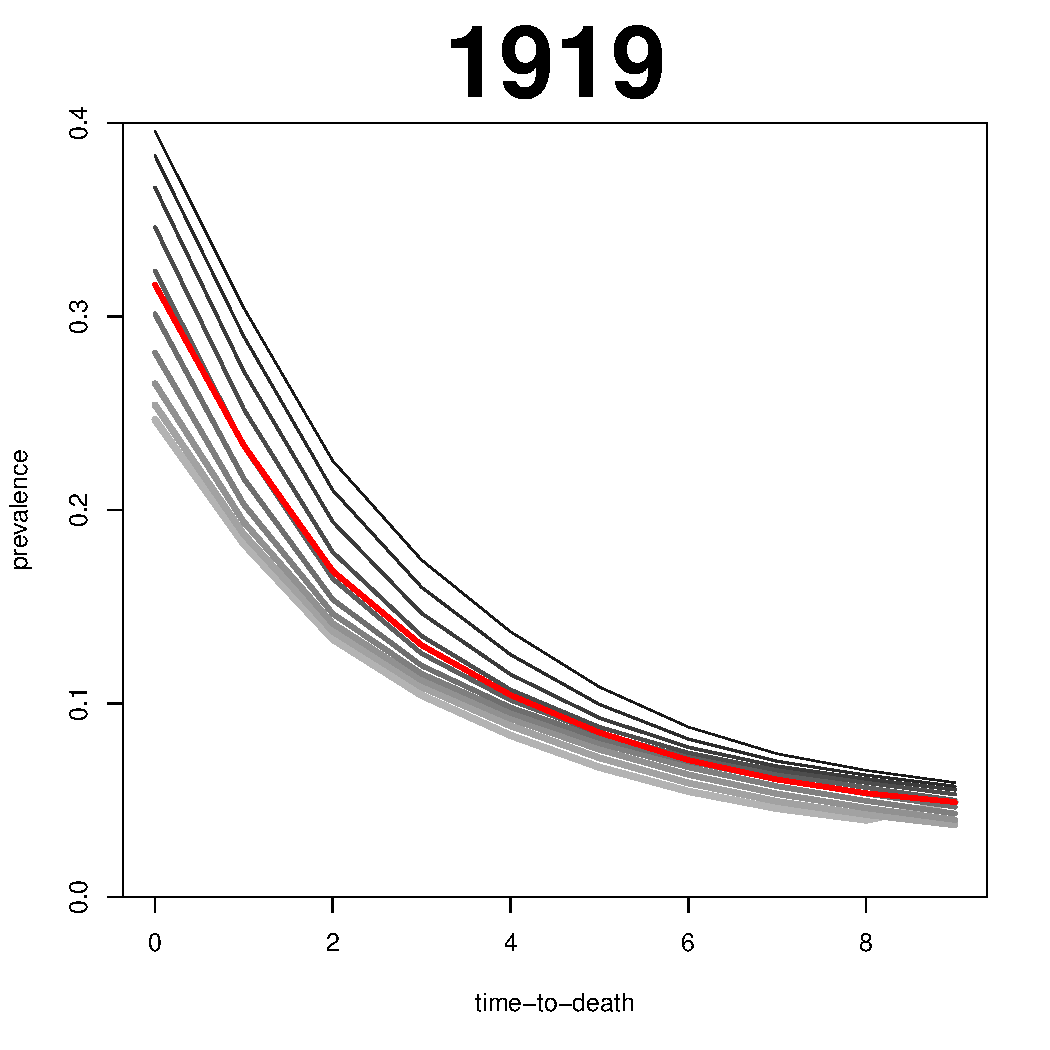
\includegraphics[width=.7\linewidth]{Figures/adl31919.pdf}}; 
    \node<6>  (img6) {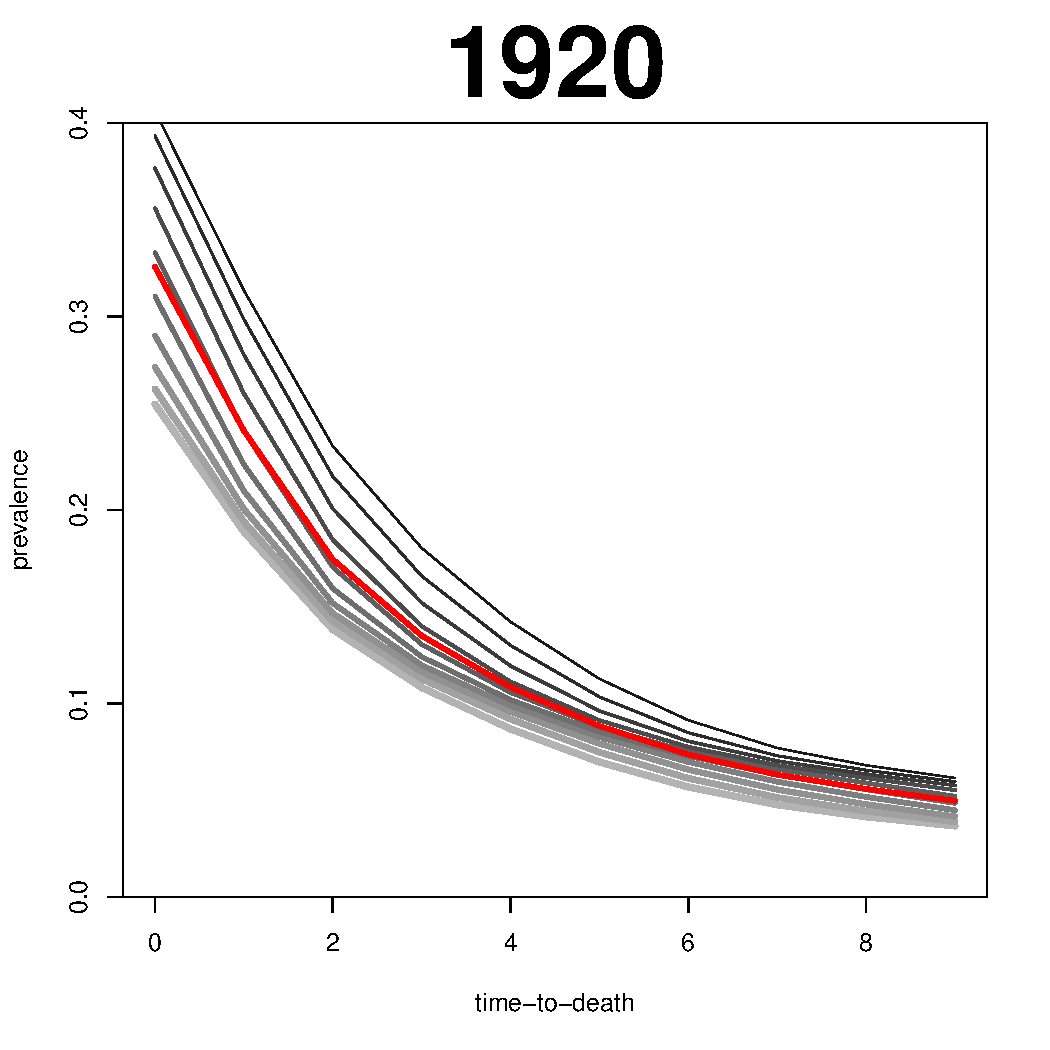
\includegraphics[width=.7\linewidth]{Figures/adl31920.pdf}}; 
    \node<7>  (img7) {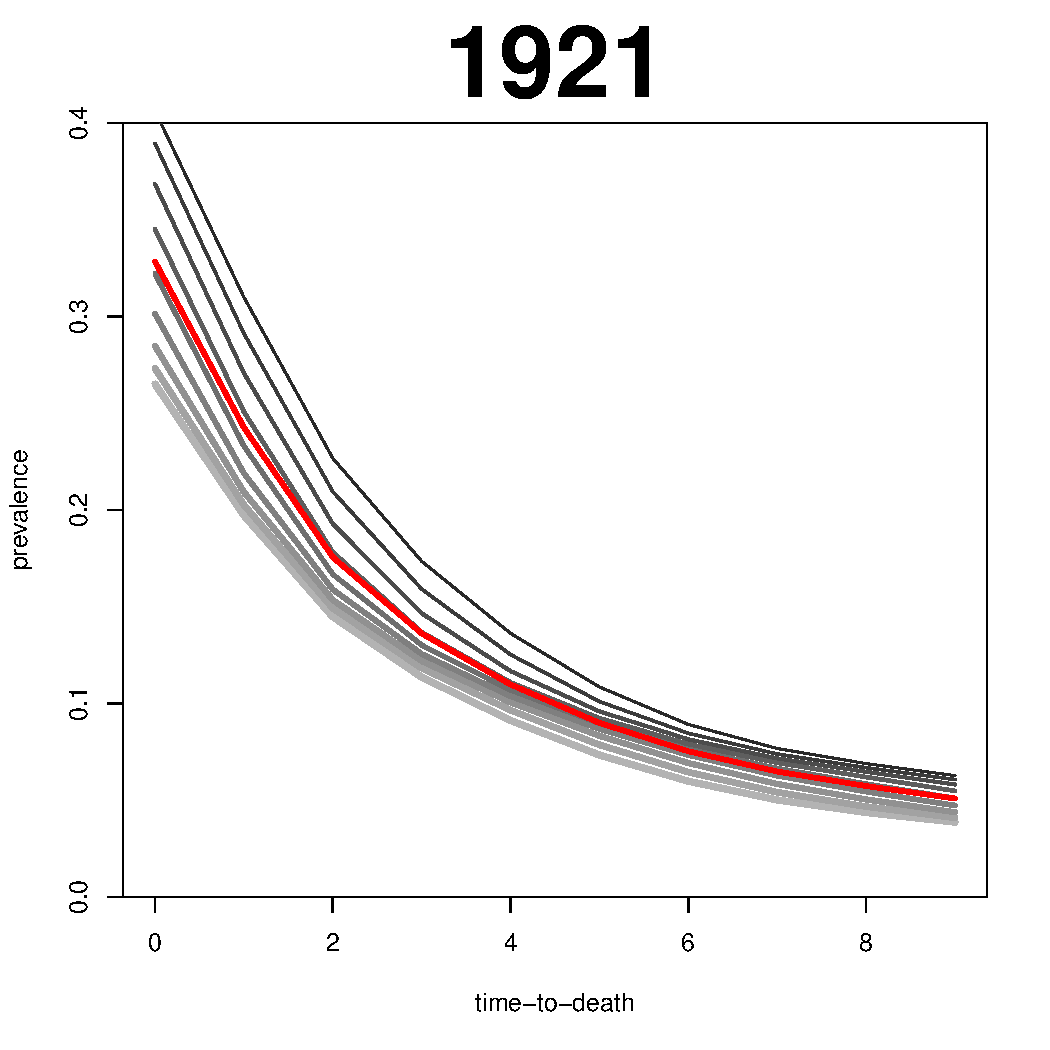
\includegraphics[width=.7\linewidth]{Figures/adl31921.pdf}}; 
    \node<8>  (img8) {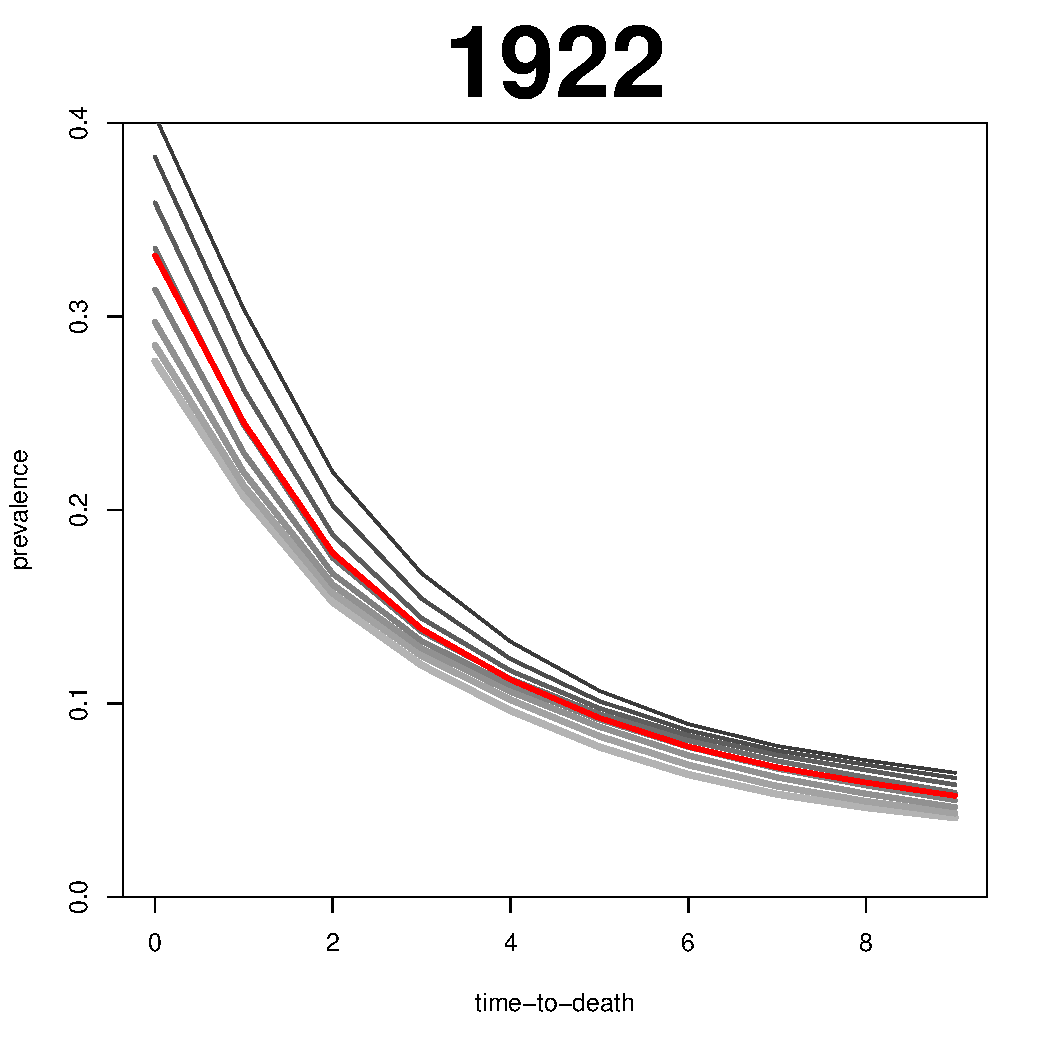
\includegraphics[width=.7\linewidth]{Figures/adl31922.pdf}}; 
    \node<9>  (img9) {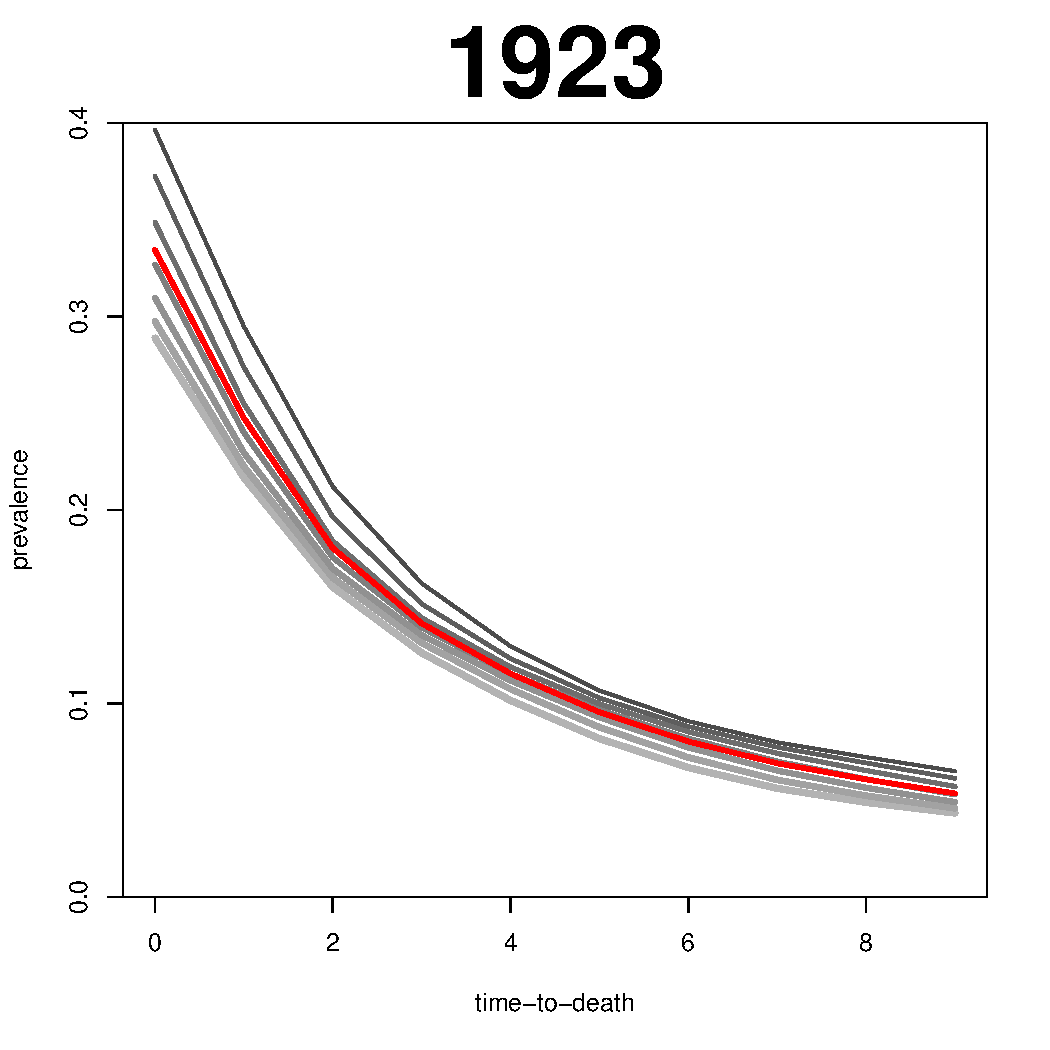
\includegraphics[width=.7\linewidth]{Figures/adl31923.pdf}}; 
    \node<10> (img10) {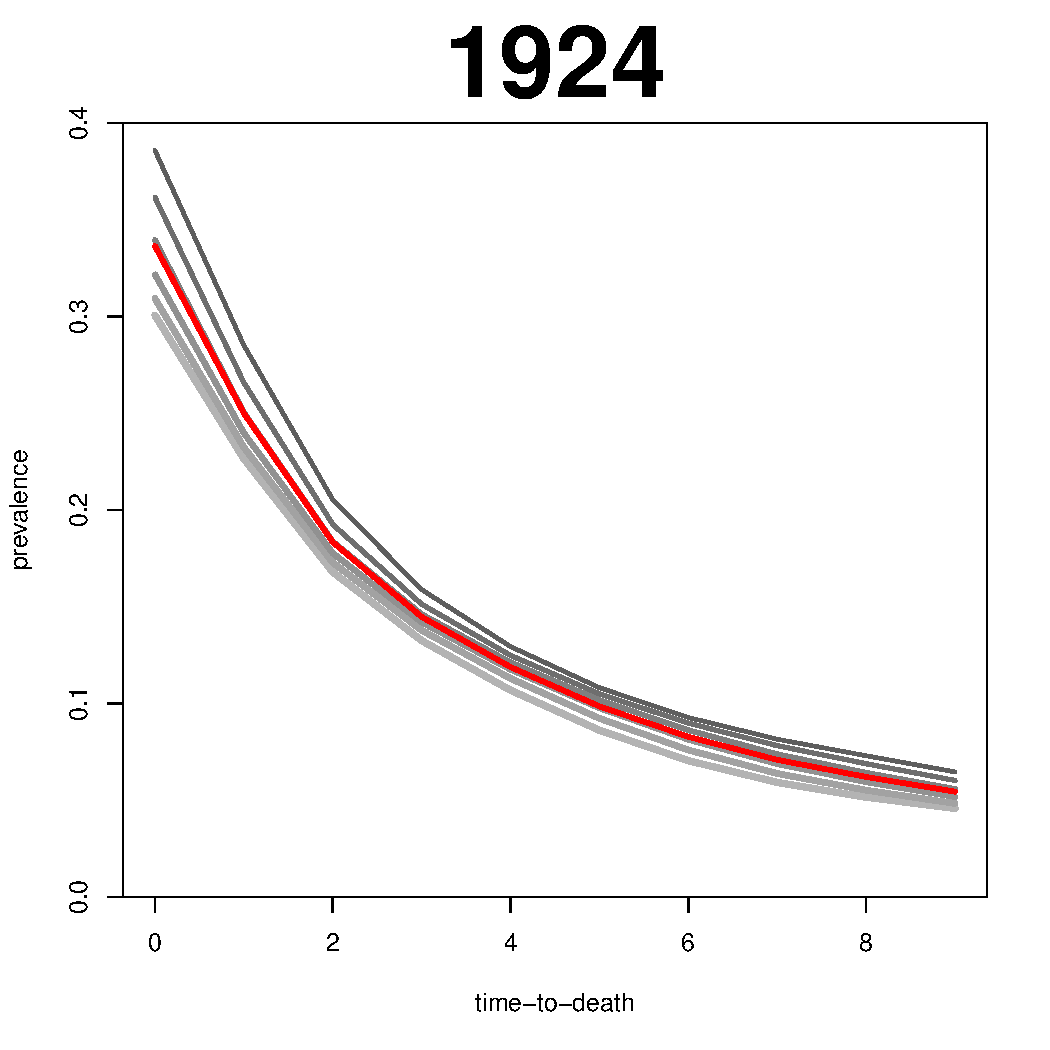
\includegraphics[width=.7\linewidth]{Figures/adl31924.pdf}}; 
    \node<11> (img11) {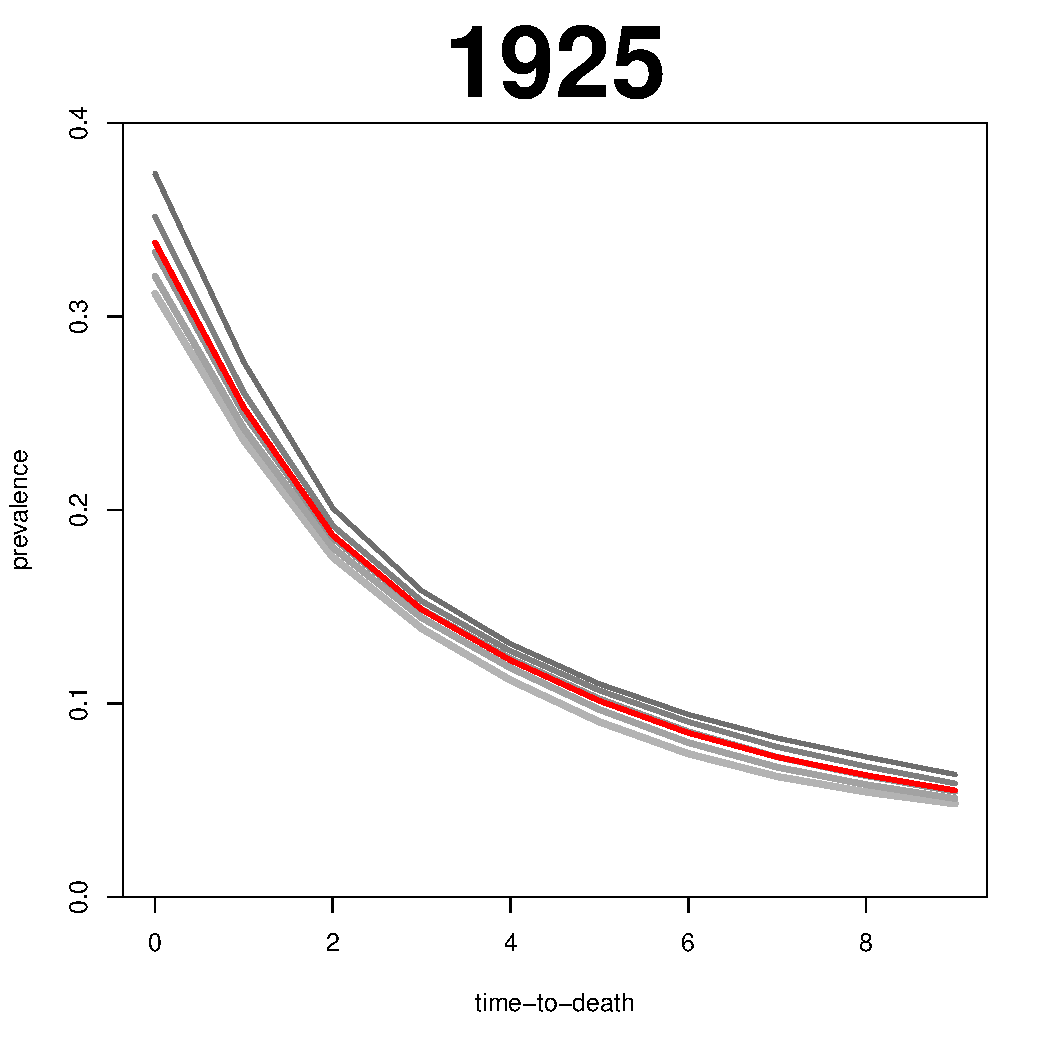
\includegraphics[width=.7\linewidth]{Figures/adl31925.pdf}}; 
  \end{tikzpicture}
\end{center}
\end{frame}

\begin{frame}
\frametitle{ \boldmath$\overline{TTD}$ patterns, psych problems and ADL3}
\begin{center}
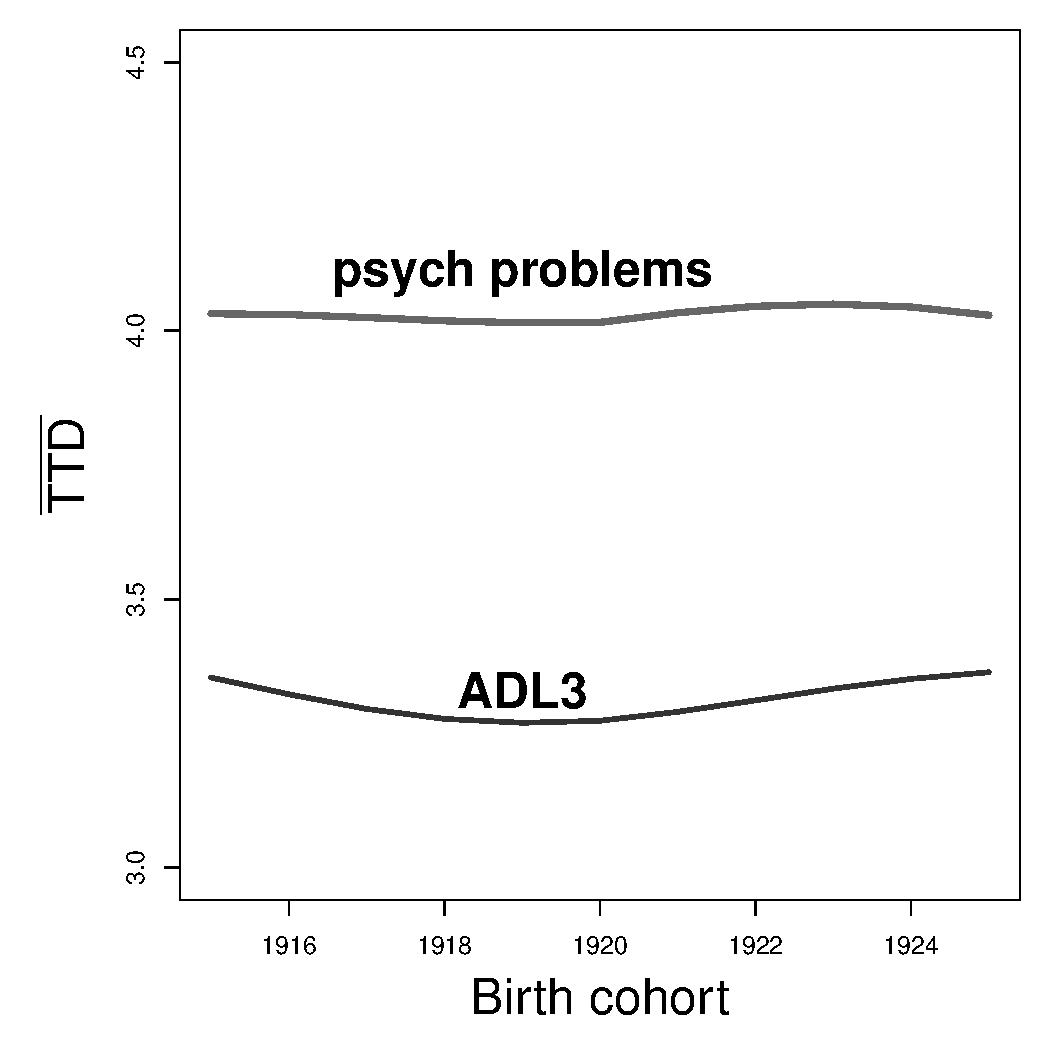
\includegraphics[scale=.9]{Figures/TrendsMeanTTD.pdf}
\end{center}

\end{frame}



%----------------------------------
%%%%%%%%%%%%%%%%%%%%%%%%%%%%%%%%%%
%%	End of the document			%%
%%%%%%%%%%%%%%%%%%%%%%%%%%%%%%%%%%
\end{document}










